%!TEX root = ../../thesis.tex
%!TEX enableSynctex = true
%*******************************************************************************
%*********************************** First Chapter *****************************
%*******************************************************************************

\ifpdf
    \graphicspath{{Chapters/intro/Figs/Raster/}{Chapters/intro/Figs/PDF/}{Chapters/intro/Figs/}}
\else
    \graphicspath{{Chapters/intro/Figs/Vector/}{Chapters/intro/Figs/}}
\fi

\chapter{Introduction}

%
% % \noindent
% %Fluorescence microscopy has experienced a scientific renaissance over the last 20 years through advances in new fluorescent proteins and super-resolution optical microscopy, both of which were awarded with Nobel Prizes in Chemistry.
% Fluorescence microscopy is one of the cornerstones of modern biology, but has generally been limited to 2D culture dishes.
% Light-sheet microscopy, a recent advance which was awarded Nature Method of the Year 2014, allows fast, non-invasive 3D imaging across an entire organism.
% This works by decoupling illumination and detection such that the microscope only illuminates a thin section of tissue at a time.
% By scanning this `light-sheet' through an organism we can image in 3D more quickly and with less damage than other techniques such as confocal microscopy.
% %we can construct a detailed 3D image with sub-cellular resolution.
%
% %Traditional techniques are slow.
% % Super-resolution microscopy allows an improvement in optical imaging resolution previously thought to be physically impossible.
% % Super res great, but only good in 2D. %Confocal is 3D but is slow and "force entire" and isn't super res.
% % lightsheet is fast, 3D and can be supe res, by seperating objective
% %We can now visually inspect live biological specimens in real time and at protein length scales.
% %These imaging techniques do however require long acquisition and exposure times, and so force the entire biological sample to be flooded with light, which subjects delicate samples to harmful radiation.
% %Light sheet Fluorescence Microscopy is distinct from these techniques in that it introduces an additional excitation lens at right angles to the detection, confining the illumination to the plane of interest and minimising harm to the sample.
% %This decoupling then allows for fast, non-invasive 3D imaging across an entire organism.
% %This decoupling then allows for fast, deep and non-invasive volumetric imaging.
% %Light sheet Fluorescence Microscopy was Nature Method of the Year 2014 and promises to be the future standard, disrupting 400 years of established microscopy.
% %These advances have been so revolutionary that Light-sheet fluorescence microscopy was awarded Nature Method of the Year 2014.
%
% %During the first year of my PhD
% A custom light-sheet microscope was designed and built  for the application of cell mechanics of developing embryos and the tracking of viral egress.
% %Cell mechanics plays a vital role in the development of organisms;
% Internal stresses within tissues induce cellular migrations that can govern the organism's resultant anatomy.
% We have developed a technique to mechanically probe deep tissue using magnetism.
% By embedding a magnetic bead in an embryo we can use a controllable, non-invasive magnetic field to move the bead.
% By pushing a magnetic bead and allowing it to relax we can fit a model to its trajectory and so extract local mechanical properties.
% % Comparing results between embryos that are genetically modified to no longer produce different key proteins provides an understanding of their roles in embryonic development. %TODO Reword
% The mechanical roles of key proteins in embryonic development can be inferred by comparing results between genetically modified embryos.
% %Using light-sheet imaging we can rapidly visualise entire live cells, permitting an unprecedented opportunity to observe and induce cell migration and tissue formation.
% %Our investigations so far have demonstrated that rho-kinase, in embryonic development increases cell stiffness
% %is inaccurate. %and %TODO add something.+
% Our investigations so far have contradicted previous reports that rho-kinase increases cell stiffness in embryonic development. These results are currently being prepared for publication with our collaborators.
%
% % Looking ahead, I intend to  single magnetic bead tracking to that of single virus particle tracking, going from the microscopic to the nanoscopic.
% %Looking ahead, I intend to move from tracking single magnetic beads to tracking single virus particles, going from the microscopic to nanoscopic scale.
% Virus particles (virions) invade host cells and hijack their machinery to replicate and then spread. %their disease
% By visualising the journey of virions through the cell we may reveal weaknesses in infection pathways.
% %Light-sheet microscopy is the only technique capable of volumetrically tracking virions, which are both exceptionally small and fast.
% Light-sheet microscopy is better suited than other techniques for tracking virus trafficking in 3D as virions are exceptionally small and fast.
% We intend to study Herpes Simplex Virus~1 which causes cold sores and genital herpes.
% Furthermore, it serves as a biological model for other Herpesviruses which are associated with many serious diseases including chickenpox and certain lymphomas.
% %and life-threatening conditions in immuno-compromised patients.
% %Herpesvirus pathogens are ubiquitous in vertebrates and establish life-long latent infections in their hosts.
% %Infections by the nine known human herpesviruses are associated with many serious diseases including certain lymphomas and life-threatening conditions in immuno-compromised patients.
%
% In addition to designing and constructing a light-sheet fluorescence microscope I have made technological improvements which will be useful for other researchers.
% %In addition to design, construction and application, I am also contributing directly to the field of light-sheet microscopy itself.
% %So far I have proposed two improvements.
% The first is a three dimensional region-of-interest technique which promises to simultaneously simplify volumetric imaging calibration whilst also being more robust than current approaches.
% The second improvement builds upon confocal slit scanning, a technique used in our lab to increase image contrast but takes twice as long to acquire an image.
% This development now allows for full speed imaging with the same increased contrast.
% I am currently preparing two manuscripts detailing these improvements for submission to \emph{Optics Letters}.
% % Herpesviruses also cause a significant disease burden in animals that can lead to economic problems for livestock farmers.
% % In visualising HSV1 virions leaving a cell (a step which contributes directly to viral pathology but is lesser studied)
% % Specifically, we intend to track HSV1 as it exits a cell, after replication; the spreading stage
% % This aspect of viral infection is poorly understood but contributes directly to virus pathology
% % Medicines which could block a virion from exiting from a cell would inhibit the viral spread; this medical imprisonment of virions could then provide an effective, curative treatment.
% % Virions invade host cells and hijack their machinery to replicate and then spread their disease. By visualising the journey of virions through the cell we may reveal finding weaknesses in its infection pathology.
% % Specifically we intend to study Herpes Simplex Virus 1, as it begins to exit a cell and spread.
% % By understanding how virions interact with cellular machinery we can provide targeted medicine
% % By visualising the journey of virions we may reveal finding weaknesses in its infection pathology
% Light sheet microscopy is the only technique capable of tracking virons which are both exceptionally small and fast

Light-sheet microscopy is at the cutting edge of live-organism imaging.
%In the coming years it will be adopted as the standard of biological imaging and transform modern biology into a highly quantitative, multidisciplinary and exciting field.
In the coming years it will help move biology out of the petri dish and back into the animal.
Further development requires the marriage of physics, maths, statistics, computer science, chemistry and biology, in laboratories such as the Laser Analytics Group.
% I am privileged to apart of, what I believe to be, a paradigm shift in fluorescence microscopy; a field which is also highly rewarding as it marries physics, maths, statistics, computer science, chemistry and biology, a fusion I find fascinating given my physical sciences background.

%Section outlining everything


The aim of this work was to develop a light sheet microscope imaging system which permitted the three dimensional tracking of particles through biological samples.
%his will be used to monitor how toxic proteins travel between cells and
%how virus particles infect their host organisms with minimal %With the ability to image very quickly and tracking three dimensionally particulate targets (such as virus particles) with minimal
%photo-damage to the sample, using animal models such as drosophila.
This system was be based on the work of Ernst Stelzer who pioneered digital light sheet technology\cite{Huisken2004}.
A light sheet microscope uses orthogonal illumination and detection to optically section biological samples.
A previous system was built in order to study developmental biology.
This work intended to improve upon this design so as to facilitate fast 3D particle tracking.

% The new system will:
% \begin{itemize}
% 	\item Be more vibrationally stable for low noise tracking
% 	\item Accommodate a three dimensional stage for particle tracking and volume imaging with nanometre resolution
% 	\item Use structured illumination modes that can provide higher resolution than standard illumination
% 	\item Provide more excitation wavelengths to enable improved biological flexibility in terms of fluorescent dyes that can be used with better specificity
% 	\item Feature a user-friendly software interface so that users can produce images independently with a strong programming architecture for future collaborative development.
% \end{itemize}
%The new system will be designed to be: ; ; ;  and

\subsection{Motivation}
 %Other viruses are more deadly such as HIV, by understanding viruses medicine may be better equipped to cure or prevent infection.
%Viral infection and Alzheimer's are currently
Viruses are carriers of infectious disease in humans, by hijacking the internal working of the cell the virus replicates using the machinery of the cell.
\SI{80}{\percent} of adults in the UK are thought to be infected with Herpes Simplex Virus 1 (cold sores) which is currently medically incurable\cite{Herpes}; only the symptoms can be suppressed.
Understanding virus pathology is a requirement for assisting in therapeutic intervention.
The virus structure is well understood through high resolution techniques such as Atomic Force Microscopy and Electron Microscopy.
In this group we have used super resolution techniques to study the Herpes Simplex Virus 1 structure \textit{in vitro}\cite{Laine2015}.
Contemporary biological models of viral infectivity dynamics are based on \textit{in vitro} studies %; by tracking a single virus particle through its entire infection process \textit{in vivo}.
Studying these dynamics \textit{in vivo} and following a virus through its entire process in a living organism could provide new, useful insights and understanding which could be used to suppress or reverse viral infection in humans.
Virus particles are smaller than the diffraction limit  (\SI{20}{\nano\meter}-\SI{200}{\nano\meter}); optical super resolution techniques can image sub-diffraction limit and have observed Human Immunodeficiency Virus 1\cite{Pereira2012}.
Virus particles move tens of nanometres on the time scale of milliseconds\cite{Brandenburg2007}, these techniques currently do not produce the temporal resolution required to accurately track virus particles\cite{Brandenburg2007} in three dimensions and are limited to \textit{in vitro} studies.
%
% Dementia among the rapidly ageing first world population is becoming a heavy burden on healthcare; as of 2015 there are \SI{850000}{} people in the UK suffering with dementia\cite{Judd}.
% Alzheimer's disease (AD) is a neurodegenerative affliction accounting for 62\% of all dementia suffers.
% Amyloid fibril plaques and neurofibrillary tangles (NTF) are commonly found in post mortem AD sufferers' brains.
% It is believed that misfolded Amyloid plaques trigger the accumulation of neurofibrillary tangles and a toxic species of microtubule-associated protein, tau\cite{Ittner2011,King2002}.
% Within our group we have studied Amyloid fibril aggregation using super resolution techniques and the role of tau proteins in neuronal dysfunction.
% We have demonstrated that extracellular tau can initiate tau pathology in AD\cite{Michel2014a}, a complimentary \textit{in vivo} study on tau protein's\cite{DeCalignon2012} dynamic propagation in axons would serve to elucidate AD pathology.
%
% These issues can be addressed using light sheet technology.
% Light sheet microscopes use orthogonal plane illumination to optically section biological samples, allowing an \textit{in vivo} three dimensional study.
% Confocal microscopy also produces optical sectioning, however its raster scanning nature means it is a slow technique.
% Orthogonal illumination and detection allows detection rates comparable to wide-field.
% Light sheet technology is also a low photo-toxcity method compared to confocal and as such can image for extended periods of time at millisecond resolution.

Particle localisation techniques are compatible with light sheet microscopy and can be used to accurately localise particles to sub-pixel, sub-diffraction limited positions in two dimensions.
In conjunction with a novel third dimensional tracking technique, exclusive to light sheet, full sub-diffraction limited tracking is viable\cite{Spille2015a}.
This will then enable the \textit{in vivo} study of virus trafficking through a host cell and protein propagation in neurons with unparalleled temporal resolution.

%needed to track
%To localise sub-diffraction limited particles in a light sheet system in

%A new technique exclusive to light sheet technology will allow the tracking of sparse sub-diffraction limited particle


%Virus particles are carriers of infectious disease within humans.
%Virus structure sub-diffraction limit in size, the smallest being \SI{20}{\nano\meter} and \textit{human immunodeficiency virus type 1} being \SI{125\pm14}{\nano\meter}

%\textit{Herpes Simplex Virus 1}  being is well known from AFM and Electron microscopy.
%Recently super resolution techniques verified this structure aswell.
%A virus is composed

%Monitoring virus motion within a cell gives insights to the pathology and understanding of infectivity of the virus.

%TODO Motivations

%The motivation of this project is to aid the endeavours of biology through advanced imaging capability to tackle important biological questions.
%Questions involving diseases such as Alzheimer's and cancer so they can be better understood and thus curable


%Similiarly the

% is \SI{20}{\nano\meter}
%\begin{itemize}
%
%\item Viruses are carriers of infectious disease within humans
%
%
%\item Virus and spore structure statically well known using AFM and Electron beam.
%Dynamics, \textit{in vivo} less understood pathology currently monitored \textit{in vitro} and a full single virus nor spore particle has never been tracked through its entire infection process
%
%
%\item The applications of this microscope are varied and include:
%
%\item Virus and spore trafficking pathology in vivo.
%\item Tracking of molecule dynamics of neurodegenerative diseases such as Alzeihmers.
%\item (Maybe?) Development of cancers and tumours.
%
%\item Optical microscopy can be used to study these processes however, they are at a length of 10-200nm below the diffraction limit of visible light.
%Not only are these processes small but they are fast (cite).
%Super-resolution techniques exist to break the diffraction limit however, they sacrifice temporal resolution for spatial resolution.
%
%\item Localisation can track particles to precisions below the dffraction limit.
%
%\item Light sheet microscopy creates optical sectioning for three dimensional \textit{in vivo} study of these processes.
%A recent innovation in light sheet microscopy means that particles can be track axially as well as laterally, in real time and \textit{in vivo}.
%
%\item It is expected that this system will be able to accurately track virus and spore pathology \textit{in vivo} , a feat which has not yet been realised.
%
%\end{itemize}

%\subsection{Aims}


\subsection{Structure}

% Here, a light sheet microscope is developed to track particles in three dimensions with millisecond temporal resolution.
% Firstly the theory of fluorescence microscopy and light sheet microscopy is discussed with a comparison to other similar techniques followed by a review of particle tracking methods which are considered in the context of a light sheet microscope.
% The current biological model of virus pathology and tau protein propagation and their challenges is then presented.
% This report then discusses the methods and materials used to build a light sheet microscope up until its current state.
% Finally the progress of the microscope is summarised and the future work for the project is discussed in terms of experiments needed (once the system is operational) to determine its ability and limitations when applied to virus and tau protein tracking.


\chapter{Principles of fluorescence microscopy}

%Physical prciniples of the operation of a light-microscope.
%Capabilities limtiations.

\section{Light microscopy}
\subsection{Construction of light microscopes}

%Consists of illumination elements and detection elements.

\subsubsection{Components of light microscopes}
%Imaging part of microscope is formed of two leneses
%Infinity corrected system.
Light emitted by a point $o_1$ at the sample plane is transformed into a parallel ray bundle by the objective lens, which travel parallel to the optical axis.
The tube lens then refracts the ray bundle back down onto its focus.
How the ray bundle for an a point away $o_2$ from the optical axis can be determined by the \emph{chief ray} ($r_c$) which passes through the optical centre of the objective unperturbed, and the \emph{marginal ray} ($r_m$) travelling parallel to the optical axis which crosses the back-focal point of the objective lens.
Both of these rays propagate parallel in the \emph{infinity space} between the objective and tube lens, as do all sets of rays at any point $o_n$ at the focal plane of the objective lens.

\subsubsection{Magnification}

Due to the parallel propagation of rays in the infinity space the distance between the two lenses may be spaced arbitrary though typically the back focal points are matched to create a \emph{4f system}.

The marginal ($r_m'$) and chief ($r_c'$) rays incident on the tube lens then govern where a real image of the sample lies at the \emph{primary image plane}. %TODO not quite right
$o_1'$
The image size ($I$) in the primary image plane is distance between the intersection of the primary image plane to the intersect of the the margin ($r_m'$) and chief rays ($r_m'$) at the tube lens.

\begin{align}
    \tan \alpha &= \frac{O}{f_{\text{objective}}} =  \frac{I}{f_{\text{tube lens}}} \\
    \intertext{It follows that the magnification of the sample is:}
    \implies M &= \frac{I}{O} = \frac{f_{\text{objective}}}
{f_{\text{tube lens}}}
\end{align}


% Tube lens may also be used to correct for image abberations

%Great advantage is that the lgiht path behind the objective only contains paralel light, means can add optical elements without distortions the beam path.

% Other adsvantage is you can focus by moving the objective lens

%and the overall magnification of the





%\subsubsection{Magnification}

\subsubsection{Field of view}

The observable objective field (FOV) is limited by the aperture stop of the system typified as the field number ($F_n $) and the objective lens magnification $M_{\text{object}}$:
%The maximum field of view ($F_{n}$)available is by :

\begin{align}
FOV = \frac{F_{n}}{M_{\text{object}}}
\end{align}

The field number of objective lenses is limited by the image degradation caused by optical aberrations, with modern objective technology reaching up to \SI{28}{\milli\meter} from the previous standard of \SI{20}{\milli\meter}.

\subsubsection{Illumination}

The illumination system defines the contrast mode, the resolution of the instrument, and the overall brightness.
Two principally different optical setups are in use.
The simpler one is the source focus or critical illumination and the other, which is by far more prevalent, is called Köhler illumination.

Critical illumination uses a single \emph{condenser} lens whereas Kohler illumination uses a \emph{collector} lens as well.
The use of two illumination lenses allows for a conjugate 4f system of illumination to the detection optics, this ensures that all ray bundles passing through the sample are parallel and the illumination brightness is homogenous.
Having a conjugated illumination also allows for alternative contrast methods to be implemented. %TODO sort

In the illumination beam paths discussed earlier, the specimen is placed between the light source and the objective lens.
In many cases, however, it is advantageous to illuminate the specimen from the side of observation (\emph{epi-illumnination}), for instance, when looking at the reflection of opaque or fluorescent samples.
In that case, some optical components of illumination and imaging are identical, for example, the objective lens. %TODO reword


\subsection{Resolution}

%Magification versus resolution

Resolution refers to the level of detail that can be recognized in an image, such as small and intricate structures or the distance between closely placed small objects.
Indeed, such a distance is used to define and quantify the optical resolution.
Using light microscopy, minute objects can be discriminated from each other when they are positioned at a minimum distance of -0.25 mum from each other and green light and a high-quality oil-immersion objective lens are used.
This obviously means that proteins and supramolecular complexes occurring in living cells cannot be recognized in detail.
In later chapters, we discuss how the principal optical resolution limit can be overcome or circumvented by advanced optical techniques.

%Bragg conditions
%

\begin{align}
    d \sin \alpha_n = n \lambda \\
    \sin\alpha_n = \frac{p_n}{f} \\
    p_n = \frac{n\lambda f}{d} \\
    d \le = \frac{\lambda}{\sin\alpha_{\text{max}}} \\
    d \le = \frac{\lambda_0}{n\sin\alpha_{\text{max}}} = \frac{2\lambda_0}{NA}
\end{align}

\subsubsection{Angular and numerical aperture}

%An objective lenses is limited by
The maximum acceptance angle ($\alpha$) of an objective lens limits the amount of light that can be collected from the sample.
An objective lens at the may be approximated to applying a Fourier transform of the imaging space, through an aperture with radius $a$ with an imaging plane at the far field.
This leads to high frequency information being omitted during the imaging process and the microscope behaving as a low-pass filter.
The electric field ($E(r)$) and resultant intensity ($I(r)$) distribution of a single point (delta function) at the image plane then becomes:

\begin{align}
    E(r) &\propto E_0 \frac{J_1 \left(2\pi r \sin \frac{\alpha}{\lambda}\right)}{2\pi r \sin \frac{\beta}{\lambda})}\\
    \implies
    I(r) &= I_0 \left[\frac{J_1 \left(2\pi r \sin \frac{\alpha}{\lambda}\right)}{2\pi r \sin \frac{\alpha}{\lambda})}\right]^2
\end{align}

Where $J_1$ is a Bessel function of the first kind and $\beta$ is the half opening angle of the tube lens.

\subsubsection{Lateral resolution}

Point emitters are therefore imaged more faithfully with a wider collecting angles and with higher frequency light.
By placing two point emitters close such that the first zero crossing of the Bessel junction $J_1$ coincides with the centre of the second point emitter gives a distance of:

\begin{align}
    r_0,\text{objective} &\approx \frac{0.61\lambda}{n\sin\alpha} = d_r \\
    \implies d_r &= \frac{1.22 \lambda}{NA_{\text{objective}}}
\end{align}

The resulting distance is Rayleigh's criterion for resolution which provides a limit to the resolution of a system based on a dip in intensity maxima, between two neighbouring emitters, of $\sim 75\%$.

%Coherent and incoherent
\subsubsection{Axial resolution}

The Airy Disk describes the in-plane of lateral intensity distribution, with an analogous analytical function propagating axially.
Once again, by comparing the the distance to the first zero in intensity along $z$ an analytical definition can be formed:

\begin{align}
    z_0,\text{objective} = \frac{2n\lambda}{NA^2} \label{eq:}
\end{align}

The achievable axial resolution is governed by axial extension of the PSF as is $2z_0,\text{objective}$ and commonly called the \emph{depth of field} ($D\text{objective}$).
he depth of field is the distance a focussed object may be moved axially before losing image fidelity to defocus.


Depth of field

\subsubsection{Depth of field}


\subsubsection{Sampling}

Once transmitted, image information is typically recorded digitally using using a CCD camera or similar device.
According to Nyquist sampling theory the resolution of the detector required to resample the image information faithfully is $d_\text{detector} = \frac{d_r}{2}$.
To then choose the correct system magnification ($M_\text{system}$) it follows that:

\begin{align}
    M_\text{system} = \frac{2d_\text{detector}}{d_r}
\end{align}

For a detector with \SI{6}{\micro\meter} pixels a magnification on the order of $50\times$ is therefore sufficient for diffraction limited imaging using visible light.
Magnifications in excessive of this limit are deemed \emph{empty magnification} and decrease the overall SNR of the recorded image.

Over-sampling plays an important role in super-resolved systems where the additional pixel information, though diffraction limited may be used computationally to increase resolution.

% 
% \subsubsection{Light collection efficiency}
%
% To calculate the the collecting efficiency of a lens, a single radiating source is considered, a Lambert radiator.
% The flux collected is proportional to the spherical segment carved out by the lens.
%


\section{Fluoresence microscopy}
\subsection{Contrast in optical microscopy}
% Phase contrast, dark field
\subsection{Fluoresence}

\begin{figure}
    \centering
    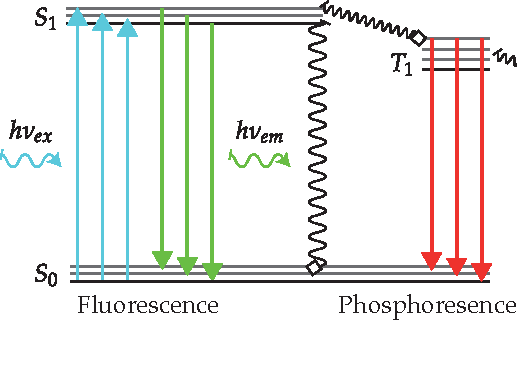
\includegraphics[width=0.7\linewidth]{jablonski_triplet}
    \caption[Standard jablonski diagram]{Jablonski diagram representing in colour the excitation of Alexa Fluor\(^{\copyright}\) 488 in a standard two level fluorescent system.}\label{fig:jablonski}
\end{figure}

\subsubsection{Spectra}
\subsection{Benefits of fluorescence microscopy}
\subsubsection{Image contrast}
\subsubsection{Specificity}
\subsubsection{Sensitivity}
\subsubsection{Illumnination}
\subsection{Signal collection}
\subsubsection{Detectors}
%ICCD
%sCMOS, CMOS
%PMT, APD
%EMCCD
\subsubsection{Noise}
\subsection{Limits of fluorescence microscopy}
\subsubsection{Photobleaching}
\paragraph{Reversible photobleaching}
\subsubsection{Phototoxicity}
\subsection{Resolution}
\section{Three dimensional fluorescence microscopy}
\subsection{Confocal Microscopy}
\subsubsection{Principles of confocal microscopy}
\subsubsection{Spinning disk confocal microscopy}
\subsection{Two photon (2P) microscopy}
\subsection{Structured illumination microscopy}
%Fast widefield 3D technique.
\subsection{Selective plane illumination microscopy}
